\chapter{Garbage collected Programming Languages}

In this chapter, garbage collection implementations of two programming
languages are presented. Both make use of the theoretical concepts presented
in \autoref{sec:overview}.

\section{Go}

Go uses a tri-color, concurrent mark \& sweep garbage collector based on an
algorithm introduced by Dijkstra in 1978 \cite{dijkstra-gc-1978}. The go
compiler employs \textit{escape analysis} for reducing the amount of heap
allocated objects at compile time (see \autoref{sec:escape_analysis}). Mark \&
sweep garbage collection introduces the requirement of tracing all memory
before any memory can be released \cite[The GC cycle]{go_gcguide_2022} for
there could still be untraced pointers marking an object previously thought to
be unreachable as reachable. This segments the gc cycles into \textit{marking}
and \textit{sweeping} while also introducing the \textit{off} phase notating
the garbage collector as inactive while no GC related work is required.

\subsection{Detecting reachable objects}

As the name suggests and introduced in \autoref{sec:gc_mark_sweep}, the go
garbage collector determines whether or not an object is to be considered
reachable by starting from the root objects (see
\autoref{sec:categorizing_memory}) and scanning all following pointers and
objects - this process is defined as the \textit{mark} stage of the mark \&
sweep algorithm.

As previously introduced, the employed algorithm for archiving this in an
efficient way is based upon the previous work by Dijkstra. This approach
revolves around three sets: the white set - all candidates for having their
memory recycled, the black set - all objects without references to the white
set and that are reachable from the roots, the grey set - objects reachable
from the roots not yet scanned for references to the white objects. Considering
this assumption, the algorithm considers all objects as white at the start of
the given garbage collection cycle and starts the following process:

\begin{enumerate}
    \item An object from the grey set is picked.
    \item Each white object the current object references is moved to the grey
        set (neither the object nor all referenced objects can be garbage
        collected) 
    \item The current object is moved to the black set.
    \item Repeat previous steps until the grey set is empty.
\end{enumerate}

This algorithm has the advantage of allowing ``on-the-fly'' garbage collection
without halting the whole system for long time periods, therefore reducing the
latency typically imposed onto systems by garbage collection
\cite[Abstract]{dijkstra-gc-1978}. This is implemented by marking objects as
soon as they are allocated and during their mutation, thus maintaining the
previously introduced sets. The garbage collector can monitor the set sizes and
clean up periodically, instead of doing so as soon as its required. This
approach allows for skipping the scan of the whole allocated heap on each
garbage collection cycle \cite[6. A Fine-Grained Solution]{dijkstra-gc-1978}.

\subsection{Removing unreachable objects}

\subsection{Fine-tuning}

The go garbage collector can be tweaked to fine-tune the trade-off between the
garbage collectors CPU and memory usage \cite[The GC
cycle]{go_gcguide_2022}. This can be done by invoking the go runtime with an
environment variable called \texttt{GOGC} \cite[GOGC]{go_gcguide_2022}.

The go garbage collector tries to finish a collection cycle before the current
total heap size is bigger than the target heap size.

\begin{equation}
    \textrm{Target heap memory} = \textrm{Live heap} + \left(\textrm{Live heap} + \textrm{GC roots}\right) \cdot \textrm{GOGC} / 100
\end{equation}

For the given values of a live heap size of 8 MiB\footnote{MiB: 1024 Kibibytes}, 1 MiB of goroutine stacks,
1 MiB of pointers in global variables and a value of 100 for the \texttt{GOGC}
environment variable the equation results in:

\begin{align}
    \textrm{Target heap memory} &= 8 \ \textrm{MiB} + \left(8 \ \textrm{MiB} + 1 \ \textrm{MiB}\right) \cdot 100 / 100 \\
                                &= 17 \ \textrm{MiB}
\end{align}

This formula allows for a precise garbage collection cycle trigger, such as
running a garbage collection cycle once the specific threshold of newly
allocated memory, here the 10 MiB cumulated from the 8 MiB live heap, 1 MiB
goroutine stack and 1 MiB global variables. The \texttt{GOGC} variable controls
this threshold. A value of 100 signals the garbage collector to switch into the
marking stage once 100\% of the size of previous live heap is allocated since
the last garbage collection cycle, a value of 50 halves the threshold from 10
MiB to 5 MiB, the value 200 doubles the threshold to 20 MiB
\cite[GOGC]{go_gcguide_2022}.

\section{Java}

Java by default uses a generational garbage collector as introduced in
\autoref{sec:gc_generational}. This garbage collector is called Garbage First
(G1) and was made the default with Java 9 \cite{java_gc_comparison_2018}.
Before that, Java used various types of mark and sweep collectors
\cite{java_available_gcs}.

Beyond those there are many more garbage collectors available for Java that can
be used by specifying them as a command line argument to the JVM. These are not
relevant for this writing, as they are not used by default. Nonetheless these
can be very useful when wanting to use a garbage collector tuned to a specific
use case.

\subsection{Garbage First Collector introduction}

Contrary to the theoretical concept of a generational garbage collector introduced in \autoref{sec:gc_generational},
the memory areas for each generation in G1GC are not continuous in memory.
Instead G1GC uses a heap divided into regions usually 1 MB - 32 MB in size.
Each region is assigned to one of the generations or unused.
These generations are called Eden, Survivor and Old. \cite{java_g1_getting_started}
An example heap layout with regions assigned to the generations is shown in \autoref{fig:g1_heap_layout}.

\begin{figure}[htbp]
    \centering
    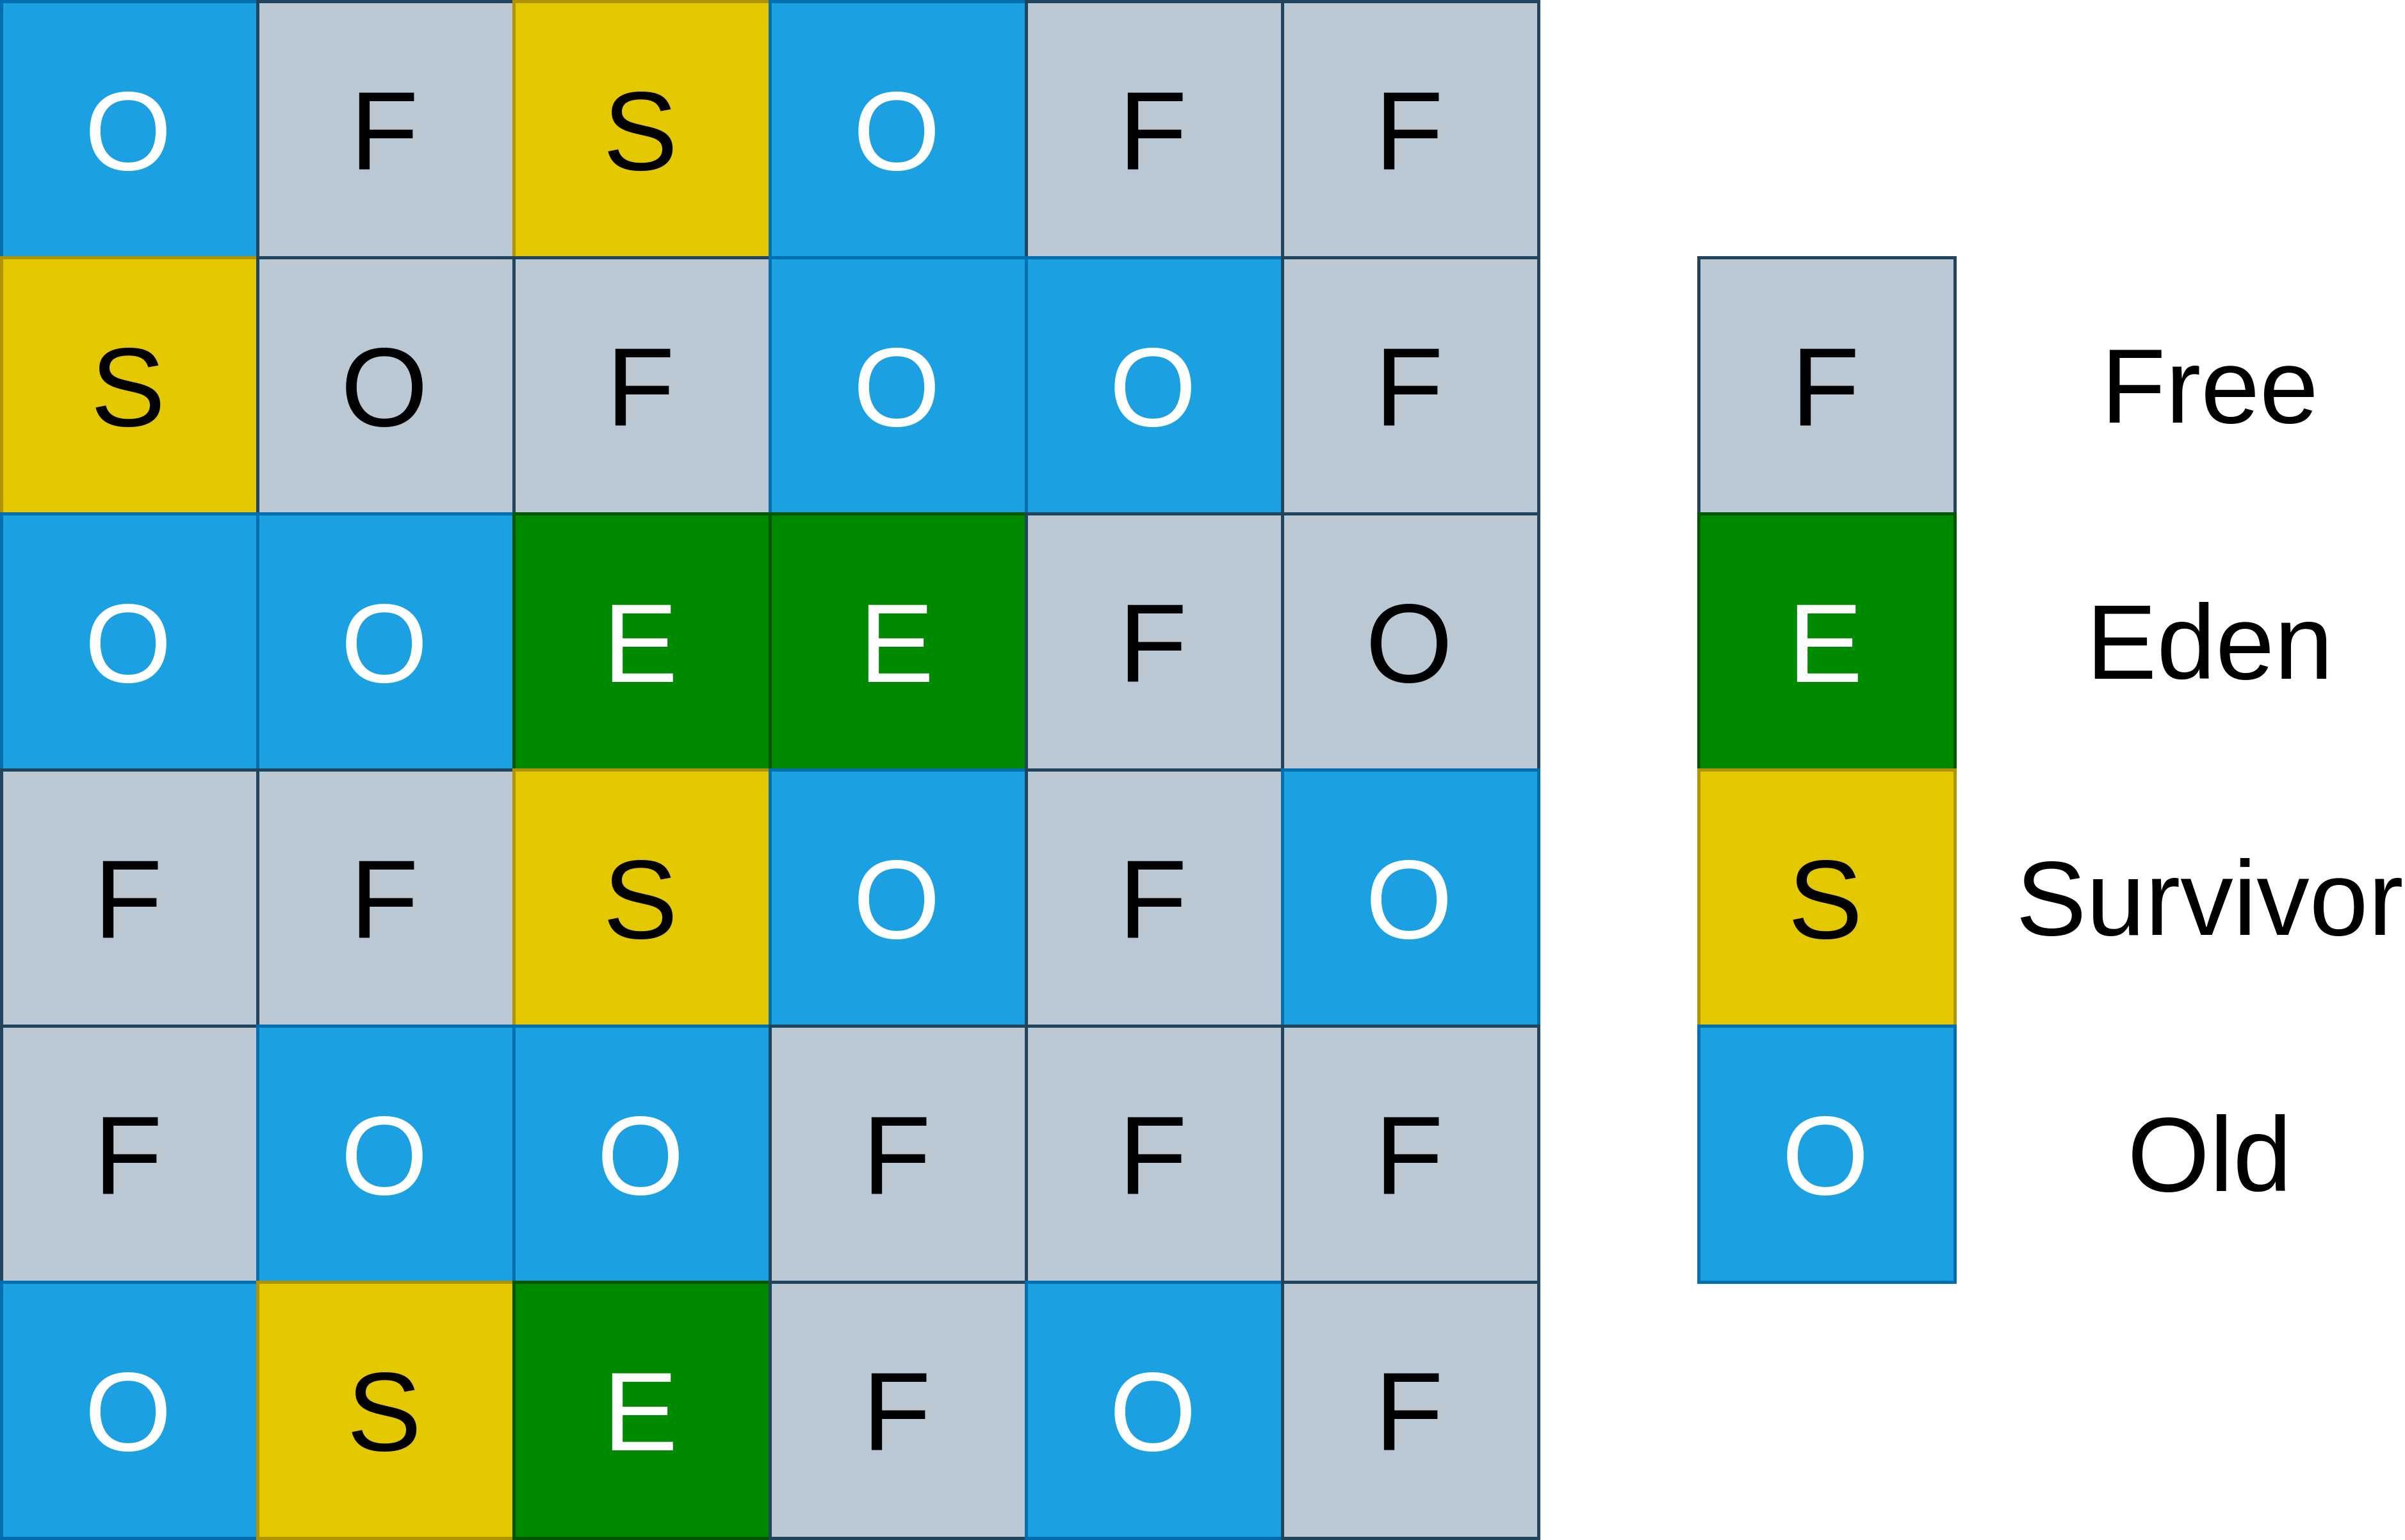
\includegraphics[width=.7\textwidth]{images/G1_Heap_Layout.drawio.png}
    \caption{Heap layout of the G1 garbage collector}
    \label{fig:g1_heap_layout}
\end{figure}

Using constant sized regions instead of continuous memory areas has the advantage
that the heap does not need to be contiguous in memory for generational garbage collection to work.

\subsection{Allocating memory to new objects}

When a object is allocated onto the heap, it will be first allocated into the
Eden region inside of the Young generation as outlined in the theoretical concept
of generational garbage collection in \autoref{sec:gc_generational}.
One memory region is marked as the current allocation region.
New objects are allocated into this region until.
Once the region is full, it will be marked as full and a new currently unused region will be
chosen as the new allocation region \cite[2.1 Allocation]{java_g1_2004}.
If no free memory region is available, a new one will be allocated through the operating system.

Large objects are stored in their own regions, called humongous regions
and not inside the Young/Old generation regions.
This is done to simplify the garbage collection of large objects which
would cause problems when stored inside the Young/Old generation regions \cite[2.1 Heap Layout]{java_g1_2004}.

\subsection{Collecting memory from memory regions}

Garbage collection is done in two phases, like outlayed in \autoref{sec:gc_tracing}.
For G1 these phases work a bit differently because of the split heap into constant size regions.

\subsubsection{Marking}

When garbage collection is triggered G1 first needs to determine
which memory regions are not referenced by any live objects anymore.
To do this G1 uses a concurrent marking algorithm that 
uses snapshot-at-the-beginning \cite[2.5 Concurrent Marking]{java_g1_2004}.
To ensure memory consistency during the marking phase, G1 uses a write barrier
to save write operations to a log.
The changes of this log are applied in the final phase of the marking phase
which will stop-the-world to apply the log changes to the heap
and retrace anything that might have changed during the marking phase \cite[2.2 Remembered Set Maintance]{java_g1_2004}.

From the traced memory regions, G1 will then select regions to collect.
This is done by estimating the amount of garbage in each heap memory region using the marking step results.
Regions with more garbage will be prioritized for collection over regions with less garbage,
because collecting regions with more garbage will result in more memory being freed for less work \cite[2.5 Concurrent Marking]{java_g1_2004}.

\subsubsection{Evacuation}

After deciding which regions to collect, G1 will start the evacuation phase.
In this phase, G1 will copy all live objects from the selected regions to other regions.
This can be either a new memory region or one that is only partly filled.
After copying all live objects, the old memory regions will be freed resulting
in the unused memory regions being freed.
Objects will be copied to regions of the same generation as the region they were copied from
or one generation older, if the objects are old enough.
The objects are copied sequentially into the new region without any gaps between them,
resulting in a compacted memory region \cite[2.3 Evacuation Pauses]{java_g1_2004}.

\subsection{Realtime goal of G1}

G1 tries have low pause times for garbage collection improving the
responsiveness of the application and allow for usage in applications
requiring predictable pause times. However pause times are only goals,
and there are no guarantees that they will be met
\cite[3.2 Satisfying a Soft Real-Time Goal]{java_g1_2004}.

It does this by estimating the amount of garbage in each region and
prioritizing regions with more garbage for collection, resulting in lower stop-the-world mark phases
compared to regions with less garbage. % TODO: source
Additionally it predicts how long a collection of a region will take and
limit the amount that is done in a garbage collection cycle to meet a
specified time goal \cite[3.2.1 Predicting Evacuation Pause Times]{java_g1_2004}.

The pause time goal and desired intervals for garbgage collection pauses can be configured using
JVM command line arguments \cite[Ergonomic Defaults for G1 GC]{java_g1_getting_started}.

